\documentclass[../notes.tex]{subfiles}

\pagestyle{main}
\renewcommand{\chaptermark}[1]{\markboth{\chaptername\ \thechapter\ (#1)}{}}
\setcounter{chapter}{7}

\begin{document}




\chapter{Many-Body Systems}
\section{The Many-Body Problem}
\begin{itemize}
    \item \marginnote{11/1:}Announcements.
    \begin{itemize}
        \item Exam room locations are on Canvas.
        \item Notice that we skipped \textcite{bib:KibbleBerkshire}, Chapter 6.
    \end{itemize}
    \item Recap: 2-body systems.
    \begin{itemize}
        \item In such a system, we have two particles: $m_1,\vec{r}_1$ and $m_2,\vec{r}_2$. Their mass sum is $M=m_1+m_2$, their center of mass is at $\vec{R}=(m_1\vec{r}_1+m_2\vec{r}_2)/(m_1+m_2)$, their reduced mass is $\mu=m_1m_2/(m_1+m_2)$, and their relative position is $\vec{r}=\vec{r}_1-\vec{r}_2$.
        \item Under a constant external force, their EOMs uncouple into $M\ddot{R}_i=Mg_i$ and $\mu\ddot{r}_i=-\pdv*{V_\text{int}}{r_i}$ where $V_\text{int}(\vec{r})$ is the interaction potential energy.
        \item Jerison will now give a better answer to last time's question, "what is the reduced mass?"
        \begin{itemize}
            \item Let's look at two important cases to start.
            \begin{enumerate}
                \item If $m_1=m_2$, $\mu=m_1/2=m_2/2$ and the particles are maximally affecting each other.
                \item If $m_1\ll m_2$, then
                \begin{equation*}
                    \mu = \frac{m_1m_2}{m_2(1+m_1/m_2)}
                    \approx m_1\left( 1-\frac{m_1}{m_2} \right)+\text{H.O.T.}
                    \to m_1
                \end{equation*}
                where H.O.T. stands for "higher order terms."
            \end{enumerate}
            \item Additionally, as $m_1/m_2\to 0$, we have $M\to m_2$, $\vec{R}\to\vec{r}_2$, $\vec{r}_2{}^*\to 0$, $\mu\to m_1$, and $\vec{r}\to\vec{r}_1{}^*$.
            \begin{itemize}
                \item Essentially, we approach the limit of 1 body orbiting a fixed object.
                \item This justifies the approximation made in earlier chapters of the Earth orbiting a fixed sun or a satellite orbiting the fixed Earth or more.
                \item Additional consideration of $\vec{r}_2{}^*=-m_2/M\cdot\vec{r}$??
            \end{itemize}
        \end{itemize}
    \end{itemize}
    \item Today: Many-body systems.
    \begin{itemize}
        \item Lagrangian, CM frame.
        \item Rockets.
    \end{itemize}
    \item Call our particle indices $\alpha=1,\dots,N$.
    \begin{itemize}
        \item \textcite{bib:KibbleBerkshire} uses a different notation! They just say $\vec{r}_i$.
        \item The mass sum in this case is
        \begin{equation*}
            M = \sum_\alpha m_\alpha
        \end{equation*}
        \item The center of mass in this case is
        \begin{equation*}
            \vec{R} = \frac{1}{M}\sum_\alpha m_\alpha\vec{r}_\alpha
        \end{equation*}
        \item The linear momentum in this case is
        \begin{equation*}
            \vec{P} = \sum_\alpha m_\alpha\dot{\vec{r}}_\alpha
            = M\dot{\vec{R}}
        \end{equation*}
    \end{itemize}
    \item In the CM frame (still denoted $*$), we have
    \begin{equation*}
        \vec{r}_\alpha = \vec{R}+\vec{r}_\alpha{}^*
    \end{equation*}
    \begin{itemize}
        \item Moreover, within the frame, we still have $\dot{\vec{R}}{}^*=0$ and hence $\vec{P}{\,}^*=0$.
    \end{itemize}
    \item Using the above, we may define the kinetic energy for the system
    \begin{align*}
        T &= \frac{1}{2}\sum_\alpha m_\alpha\dot{\vec{r}}_\alpha{}^2\\
        &= \frac{1}{2}\sum_\alpha m_\alpha(\dot{\vec{R}}+\dot{\vec{r}}_\alpha{}^*)^2\\
        &= \frac{1}{2}\Bigg( \dot{\vec{R}}{\,}^2\sum_\alpha m_\alpha+2\dot{\vec{R}}\cdot\underbrace{\sum_\alpha m_\alpha\dot{\vec{r}}_\alpha{}^*}_{0=\vec{P}{\,}^*}+\sum_\alpha m_\alpha(\dot{\vec{r}}_\alpha{}^*)^2 \Bigg)\\
        &= \frac{1}{2}M\dot{\vec{R}}{\,}^2+\frac{1}{2}\sum_\alpha m_\alpha(\dot{\vec{r}}_\alpha{}^*)^2\\
        &= T_\text{CM}+T^*
    \end{align*}
    \item We may now define the Lagrangian for the system.
    \begin{itemize}
        \item Note that
        \begin{align*}
            V &= -\sum_\alpha m_\alpha\vec{r}_\alpha\cdot\vec{g}+V_\text{int}(\{\vec{r}_\alpha-\vec{r}_\beta\})\\
            &= -M\vec{g}\cdot\vec{R}+V_\text{int}(\{\vec{r}_\alpha-\vec{r}_\beta\})
        \end{align*}
        where $\{\vec{r}_\alpha-\vec{r}_\beta\}$ denotes the vector with all pairwise differences.
        \item Combining this result with the above, we obtain
        \begin{align*}
            L &= T-V\\
            &= \frac{1}{2}M\dot{\vec{R}}{\,}^2+M\vec{g}\cdot\vec{R}+\frac{1}{2}\sum_\alpha m_\alpha(\dot{\vec{r}}_\alpha{}^*)^2-V_\text{int}(\{\vec{r}_\alpha-\vec{r}_\beta\})
        \end{align*}
    \end{itemize}
    \item Thus, the EOMs separate into
    \begin{align*}
        M\ddot{\vec{R}} &= M\vec{g}&
        m_\alpha\ddot{r}_{\alpha_i}{}^* &= -\pdv{V_\text{int}}{r_{\alpha_i}{}^*}
    \end{align*}
    where we have three of these, one for each $i=q_1,q_2,q_3$ component of particle $\alpha$.
    \item Moreover, we get two conservation laws.
    \begin{align*}
        \frac{1}{2}M\dot{\vec{R}}{\,}^2-M\vec{g}\cdot\vec{R} &= E&
        T^*+V_\text{int} &= E_\text{int}
    \end{align*}
    \item In the more general case wherein other forces act on the system, we have
    \begin{equation*}
        m_\alpha\ddot{\vec{r}}_\alpha = \sum_\beta\vec{F}_{\alpha\beta}+\vec{F}_\alpha
    \end{equation*}
    \begin{itemize}
        \item The $\vec{F}_{\alpha\beta}$ are internal pairwise forces.
        \item The singular $\vec{F}_\alpha$ represents an external force.
    \end{itemize}
    \item Linear momentum in this case.
    \begin{align*}
        \dot{\vec{P}} &= \sum_\alpha m_\alpha\ddot{\vec{r}}_\alpha\\
        &= \sum_\alpha\sum_\beta\vec{F}_{\alpha\beta}+\sum_\alpha\vec{F}_\alpha
    \end{align*}
    \begin{itemize}
        \item Since $\vec{F}_{\alpha\beta}=-\vec{F}_{\beta\alpha}$, the left term above cancels, leaving us with
        \begin{equation*}
            \dot{\vec{P}} = \sum_\alpha\vec{F}_\alpha
            = M\ddot{\vec{R}}
        \end{equation*}
        \item Recall that if there are no external forces, $\vec{P}$ is constant.
    \end{itemize}
    \item Angular momentum in this case.
    \begin{equation*}
        \vec{J} = \sum_\alpha m_\alpha\vec{r}_\alpha\times\dot{\vec{r}}_\alpha
    \end{equation*}
    \begin{itemize}
        \item It follows that
        \begin{align*}
            \dot{\vec{J}} &= \sum_\alpha m_\alpha\vec{r}_\alpha\times\ddot{\vec{r}}_\alpha\\
            &= \sum_\alpha\vec{r}_\alpha\times\sum_\beta\vec{F}_{\alpha\beta}+\sum_\alpha\vec{r}_\alpha\times\vec{F}_\alpha\\
            &= \sum_\alpha\sum_\beta\vec{r}_\alpha\times\vec{F}_{\alpha\beta}+\sum_\alpha\vec{r}_\alpha\times\vec{F}_\alpha
        \end{align*}
        \item If $\vec{F}_{\alpha\beta}$ are central (i.e., parallel to $\vec{r}_\alpha-\vec{r}_\beta$), then the left term above is zero.
        \item This leaves us with
        \begin{equation*}
            \dot{\vec{J}} = \sum_\alpha\vec{r}_\alpha\times\vec{F}_\alpha
        \end{equation*}
        i.e., $\dot{\vec{J}}$ is only affected by external forces in the central $\vec{F}_{\alpha\beta}$ case.
        \item Thus, if $\vec{F}_\alpha=0$, $\vec{J}$ is constant.
        \item Additionally, if $\vec{F}_\alpha$ are central, then $\vec{J}$ is constant because the cross product cancels.
    \end{itemize}
    \item In the CM frame\dots
    \begin{itemize}
        \item Recall that $\vec{r}_\alpha=\vec{R}+\vec{r}_\alpha{}^*$.
        \item Thus,
        \begin{align*}
            \vec{J} &= \sum_\alpha m_\alpha(\vec{R}+\vec{r}_\alpha)\times(\dot{\vec{R}}+\dot{\vec{r}}_\alpha)\\
            &= \left( \sum_\alpha m_\alpha \right)\vec{R}\times\dot{\vec{R}}+\underbrace{\left( \sum_\alpha m_\alpha\vec{r}_\alpha{}^* \right)}_{0=\vec{R}{\,}^*}\times\dot{\vec{R}}+\vec{R}\times\underbrace{\left( \sum_\alpha m_\alpha\dot{\vec{r}}_\alpha{}^* \right)}_{0=\vec{P}{\,}^*}+\sum_\alpha m_\alpha\vec{r}_\alpha{}^*\times\dot{\vec{r}}_\alpha{}^*\\
            &= M\vec{R}\times\dot{\vec{R}}+\vec{J}{\,}^*
        \end{align*}
        where
        \begin{equation*}
            \vec{J}{\,}^* = \sum_\alpha m_\alpha\vec{r}_\alpha{}^*\times\dot{\vec{r}}_\alpha{}^*
        \end{equation*}
        \item It follows that
        \begin{align*}
            \dot{\vec{J}}{\,}^* &= \dot{\vec{J}}-\dv{t}(M\vec{R}\times\dot{\vec{R}})\\
            &= \dot{\vec{J}}-M\vec{R}\times\ddot{\vec{R}}\\
            &= \dot{\vec{J}}-\vec{R}\times\sum_\alpha\vec{F}_\alpha\\
            &= \sum_\alpha\vec{r}_\alpha\times\vec{F}_\alpha-\vec{R}\times\sum_\alpha\vec{F}_\alpha\\
            &= \sum_\alpha\vec{r}_\alpha{}^*\times\vec{F}_\alpha
        \end{align*}
    \end{itemize}
    \item An application of these multi-body systems: Rockets!
    \begin{itemize}
        \item Consider a rocket traveling forward at velocity $v$.
        \item To propel itself forward, it ejects mass $\dd{m}$ at a constant speed $u$ relative to the rocket.
        \item After the ejection, the mass $\dd{m}$ travels backwards at speed $v-u$ and the remaining rocket $M-\dd{m}$ travels forward at velocity $v+\dd{v}$.
        \item We have conservation of momentum in this "explosion," so
        \begin{align*}
            (M-\dd{m})(V+\dd{v})+\dd{m}(v-u) &= Mv\\
            Mv+M\dd{v}-v\dd{m}-u\dd{m}+v\dd{m} &= Mv\\
            M\dd{v} &= u\dd{m}\\
            &= -u\dd{M}\\
            \frac{\dd{v}}{u} &= -\frac{\dd{M}}{M}\\
            \frac{v}{u} &= -\ln\frac{M}{M_0}\\
            M &= M_0\e[-v/u]
        \end{align*}
    \end{itemize}
\end{itemize}



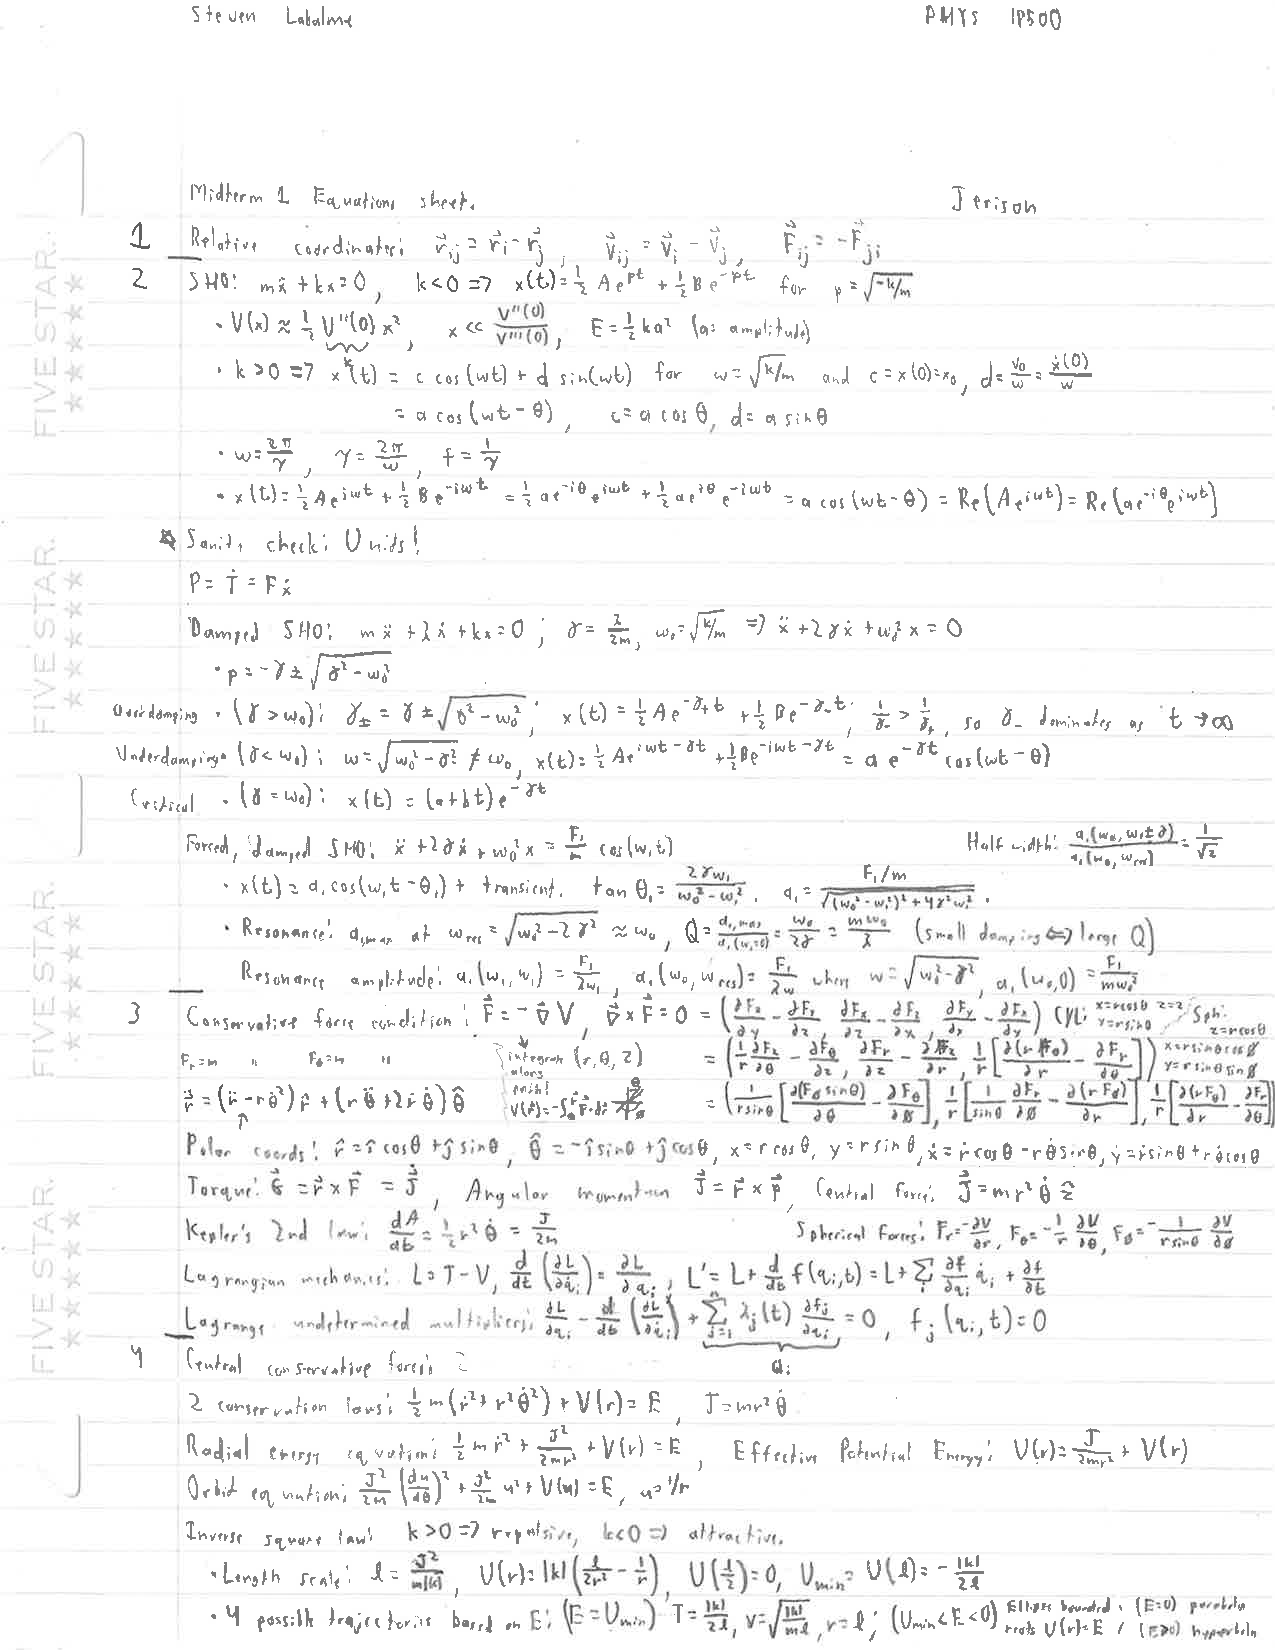
\includepdf[pages=-,addtotoc={1,section,1,Midterm 1 Equations Sheet,p1}]{../ExtFiles/Midterm1EqnSheet.pdf}



\section{Chapter 8: Many-Body Systems}
\emph{From \textcite{bib:KibbleBerkshire}.}
\begin{itemize}
    \item \marginnote{11/2:}Motivation: Studying material objects that can be regarded as "composed of a large number of small particles, small enough to be treated as essentially point-like but still large enough to obey the laws of classical rather than quantum mechanics. These particle interact in complicated ways with each other and with the environment. However, as we shall see, if we are interested only in the motion of the object as a whole, many of these details are irrelevant" \parencite[177]{bib:KibbleBerkshire}.
    \item We covered, line-for-line, Sections 8.1-8.2, and a good bit of 8.4-8.5.
\end{itemize}




\end{document}